\documentclass[t,12pt,numbers,fleqn]{beamer}
%\documentclass[t,12pt,numbers,fleqn,handout]{beamer}

\usepackage{latexsym}
\usepackage{amssymb}
\usepackage{stmaryrd}
\usepackage{phonetic}
\usepackage{wasysym}
\usepackage{pgf}
\usepackage{tikz}
\usepackage{url}
\usetikzlibrary{arrows}
\usepackage{array}
\usepackage{pgfpages} 
\usepackage{multirow} 
\usepackage{graphicx}
\usepackage{color}
\usepackage{listings}
\usepackage{hyperref}
\hypersetup{colorlinks=true,
    linkcolor=blue,
    citecolor=blue,
    filecolor=blue,
    urlcolor=blue,
    unicode=false}

\lstset{language=lisp,basicstyle=\ttfamily,breaklines=true,showspaces=false,showstringspaces=false,breakatwhitespace=true,texcl=true,escapeinside={\%*}{*)}}

%\pgfpagesuselayout{resize to}[letterpaper, border shrink=5mm,landscape] 
%\pgfpagesuselayout{2 on 1}[letterpaper,border shrink=5mm] 

\usepackage{fancybox}
%\usepackage{times}

\useoutertheme{split}

\mode<presentation>{}

%\mode<presentation>{
%\usecolortheme{whale}
%\usecolortheme{orchid}
%\useinnertheme[shadow]{rounded}
%}

%\setbeamerfont{structure}{series=\bfseries}
%\usefonttheme[stillsansseriftext,stillsansserifmath]{serif}
%\usetheme{Madrid}

\setbeamertemplate{navigation symbols}{} 
\setbeamertemplate{itemize item}[ball]
\setbeamersize{text margin left = 4mm}
\setbeamersize{text margin right = 4mm}

%% Requires:
%% 
%% \usepackage{latexsym}
%% \usepackage{amssymb}
%% \usepackage{stmaryrd}

%\setbeamertemplate{enumerate subitem}{\alph{enumii}.}

\newcommand{\be}{\begin{enumerate}}
\newcommand{\ee}{\end{enumerate}}
\newcommand{\bi}{\begin{itemize}}
\newcommand{\ei}{\end{itemize}}
\newcommand{\bc}{\begin{center}}
\newcommand{\ec}{\end{center}}
\newcommand{\bsp}{\begin{sloppypar}}
\newcommand{\esp}{\end{sloppypar}}

\newcommand{\sglsp}{\ }
\newcommand{\dblsp}{\ \ }

\newcommand{\iclicker}{i\texttt{>}clicker}

\newcommand{\sA}{\mbox{$\cal A$}}
\newcommand{\sB}{\mbox{$\cal B$}}
\newcommand{\sC}{\mbox{$\cal C$}}
\newcommand{\sD}{\mbox{$\cal D$}}
\newcommand{\sE}{\mbox{$\cal E$}}
\newcommand{\sF}{\mbox{$\cal F$}}
\newcommand{\sG}{\mbox{$\cal G$}}
\newcommand{\sH}{\mbox{$\cal H$}}
\newcommand{\sI}{\mbox{$\cal I$}}
\newcommand{\sJ}{\mbox{$\cal J$}}
\newcommand{\sK}{\mbox{$\cal K$}}
\newcommand{\sL}{\mbox{$\cal L$}}
\newcommand{\sM}{\mbox{$\cal M$}}
\newcommand{\sN}{\mbox{$\cal N$}}
\newcommand{\sO}{\mbox{$\cal O$}}
\newcommand{\sP}{\mbox{$\cal P$}}
\newcommand{\sQ}{\mbox{$\cal Q$}}
\newcommand{\sR}{\mbox{$\cal R$}}
\newcommand{\sS}{\mbox{$\cal S$}}
\newcommand{\sT}{\mbox{$\cal T$}}
\newcommand{\sU}{\mbox{$\cal U$}}
\newcommand{\sV}{\mbox{$\cal V$}}
\newcommand{\sW}{\mbox{$\cal W$}}
\newcommand{\sX}{\mbox{$\cal X$}}
\newcommand{\sY}{\mbox{$\cal Y$}}
\newcommand{\sZ}{\mbox{$\cal Z$}}

\renewcommand{\phi}{\varphi}
\newcommand{\seq}[1]{{\langle #1 \rangle}}
\newcommand{\set}[1]{{\{ #1 \}}}
\newcommand{\tuple}[1]{{( #1 )}}
\newcommand{\mlist}[1]{{[ #1 ]}}
\newcommand{\sembrack}[1]{\llbracket#1\rrbracket}
\newcommand{\bluesembrack}[1]{\bblue{\llbracket}#1\bblue{\rrbracket}}
\newcommand{\redsembrack}[1]{\bred{\llbracket}#1\bred{\rrbracket}}
%\newcommand{\sembrack}[1]{[\![#1]\!]}
\newcommand{\synbrack}[1]{\ulcorner#1\urcorner}
\newcommand{\bluesynbrack}[1]{\bblue{\ulcorner}#1\bblue{\urcorner}}
\newcommand{\redsynbrack}[1]{\bred{\ulcorner}#1\bred{\urcorner}}
\newcommand{\commabrack}[1]{\lfloor#1\rfloor}
\newcommand{\bsynbrack}[1]{\lceil#1\rceil}
\newcommand{\bsembrack}[1]{\lceil\!\!\lceil#1\rceil\!\!\rceil}
\newcommand{\mname}[1]{\mbox{\sf #1}}
\newcommand{\mcolon}{\mathrel:}
\newcommand{\mdot}{\mathrel.}
\newcommand{\modpar}{\models_{\rm par}}
\newcommand{\modreg}{\models_{\rm reg}}
\newcommand{\proves}[2]{#1 \vdash #2}
\newcommand{\notproves}[2]{#1 \not\vdash #2}
\newcommand{\provesin}[3]{#1 \vdash_{#2} #3}
\newcommand{\notprovesin}[3]{#1 \not\vdash_{#2} #3}
%\newcommand{\leqq}[1]{\mathrel{\preceq_{#1}}}
\newcommand{\parrow}{\rightharpoonup}
\newcommand{\tarrow}{\rightarrow}
\newcommand{\term}{\seq}
\newcommand{\lub}{\sqcup}
\newcommand{\subfun}{\sqsubseteq}
\newcommand{\subpred}{\subseteq}
\newcommand{\BoxApp}{\Box\,}
\newcommand{\BOX}{\mathrel{\Box}}
\newcommand{\funapp}{\mathrel@}

\newcommand{\com}{\mname{complement}}
\newcommand{\dom}{\mname{domain}}
\newcommand{\sumcl}{\mname{sum}}
\newcommand{\pow}{\mname{power}}
\newcommand{\pair}{\mname{pair}}
\newcommand{\opair}{\mname{ordered-pair}}
\newcommand{\inters}{\mname{intersection}}
\newcommand{\emp}{\mname{empty}}
\newcommand{\uni}{\mname{univocal}}
\newcommand{\fun}{\mname{function}}
\newcommand{\card}{\mname{card}}
\newcommand{\sets}{\mname{sets}}
\newcommand{\monotone}{\mname{monotone}}
\newcommand{\continuous}{\mname{continuous}}
\newcommand{\chain}{\mname{chain}}
\newcommand{\mub}{\mname{ub}}
\newcommand{\mlub}{\mname{lub}}
\newcommand{\fixedpoint}{\mname{fp}}
\newcommand{\leastfixedpoint}{\mname{lfp}}
\newcommand{\strongfixedpoint}{\mname{sfp}}
\newcommand{\emptyfun}{\triangle}
\newcommand{\statetrans}[1]{\stackrel{#1}{\longrightarrow}}
\newcommand{\thyext}{\leq}
\newcommand{\conthyext}{\unlhd}

\newcommand{\Iota}{\mbox{\rm I}}
\newcommand{\IotaApp}{\mbox{\rm I}\,}
\newcommand{\iotaApp}{\iota\,}
\newcommand{\epsilonApp}{\epsilon\,}
\newcommand{\True}{\mbox{\sf T}} 
\newcommand{\False}{\mbox{\sf F}} 
\newcommand{\Trueword}{\sf true}
\newcommand{\Falseword}{\sf false}
\newcommand{\Neg}{\neg} 
\newcommand{\Andd}{\wedge}
\newcommand{\Or}{\vee}
\newcommand{\Implies}{\supset}
\newcommand{\ImpliesAlt}{\Rightarrow}
\newcommand{\Iff}{\equiv}
\newcommand{\Sheffer}{\mathrel|}
\newcommand{\IffAlt}{\Leftrightarrow}
\newcommand{\Forall}{\forall}
\newcommand{\ForallApp}{\forall\,}
\newcommand{\Forsome}{\exists}
\newcommand{\ForsomeApp}{\exists\,}
\newcommand{\ForsomeUniqueApp}{\exists\,!\,}
\newcommand{\IsDef}{\downarrow}
\newcommand{\IsUndef}{\uparrow}
\newcommand{\Equal}{=}
\newcommand{\QuasiEqual}{\simeq}
\newcommand{\Undefined}{\bot}
\newcommand{\If}{\mname{if}}
\newcommand{\IsDefApp}{\!\IsDef}
\newcommand{\IsUndefApp}{\!\IsUndef}
\newcommand{\TRUE}{\mbox{{\sc t}}}
\newcommand{\FALSE}{\mbox{{\sc f}}}
\newcommand{\truthvalues}{\{\TRUE,\FALSE\}}
\newcommand{\LambdaApp}{\lambda\,}
\newcommand{\LAMBDAapp}{\Lambda\,}
\newcommand{\PiApp}{\Pi\,}
\newcommand{\SigmaApp}{\Sigma\,}
\newcommand{\AlphaEquiv}{\stackrel{\alpha}{=}}

\newcommand{\mvar}[3]{\textbf{var}_{#1}[#2,#3]}
\newcommand{\mterm}[2]{\textbf{term}_{#1}[#2]}
\newcommand{\mform}[2]{\textbf{form}_{#1}[#2]}
\newcommand{\mtype}[2]{\textbf{type}_{#1}[#2]}
\newcommand{\mexpr}[3]{\textbf{expr}_{#1}[#2,#3]}

\newcommand{\imps}{\mbox{\sc imps}}
\newcommand{\fol}{\mbox{\sc fol}}
\newcommand{\pf}{${\bf PF}$}
\newcommand{\pfstar}{${\bf PF}^\ast$}
\newcommand{\lutins}{\mbox{\sc lutins}}
\newcommand{\vlisp}{\mbox{\sc vlisp}}
\newcommand{\vmach}{\mbox{\sc vmach}}
\newcommand{\gnu}{\mbox{\sc gnu}}
\newcommand{\zf}{\mbox{\sc zf}}
\newcommand{\nbg}{\mbox{\sc nbg}}
\newcommand{\pnbg}{\mbox{\sc pnbg}}
\newcommand{\snbg}{\mbox{\sc snbg}}
\newcommand{\pfol}{\mbox{\sc pfol}}
\newcommand{\nbgstar}{$\mbox{\sc nbg}^\ast$}
\newcommand{\boldnbgstar}{$\mbox{\bf NBG}^\ast$}
\newcommand{\stt}{\mbox{\sc stt}}
\newcommand{\eves}{\mbox{\sc eves}}
\newcommand{\hol}{\mbox{\sc hol}}
\newcommand{\mizar}{Mizar}
\newcommand{\nqthm}{Nqthm}
\newcommand{\pvs}{\mbox{\sc pvs}}
\newcommand{\stmm}{\mbox{\sc stmm}}

\iffalse
\newtheorem{thm}{Theorem}[section]
\newtheorem{cor}[thm]{Corollary}
\newtheorem{lem}[thm]{Lemma}
\newtheorem{prop}[thm]{Proposition}
\newtheorem{rem}[thm]{Remark}
\newtheorem{eg}[thm]{Example}
\newtheorem{df}[thm]{Definition}
\fi

%\newenvironment{proof}{\par\noindent{\bf Proof\ \ }}{$\Box$}

\newenvironment{namedform}[1]
   {\begin{tabbing}\textbf{#1}\ }
   {\end{tabbing}}

\newcommand{\urlpart}[1]{\mbox{\texttt{#1}}\linebreak[0]}

\newcommand{\bblue}{\textcolor{blue!80!black}}
\newcommand{\bgreen}{\textcolor{green!55!black}}
\newcommand{\bbrown}{\textcolor{brown}}
\newcommand{\bred}{\textcolor{red!80!black}}
\newcommand{\bcyan}{\textcolor{cyan!80!black}}
\newcommand{\bmagenta}{\textcolor{magenta}}
\newcommand{\byellow}{\textcolor{yellow}}
\newcommand{\borange}{\textcolor{orange}}
\newcommand{\bviolet}{\textcolor{violet}}
\newcommand{\bpurple}{\textcolor{purple}}
\newcommand{\bdarkgray}{\textcolor{darkgray}}
\newcommand{\bgray}{\textcolor{gray}}
\newcommand{\blightgray}{\textcolor{lightgray}}

\newcommand{\clicker}{i\texttt{>}clicker}

\newenvironment{changemargin}[2]{%
  \begin{list}{}{%
    \setlength{\topsep}{0pt}%
    \setlength{\leftmargin}{#1}%
    \setlength{\rightmargin}{#2}%
    \setlength{\listparindent}{\parindent}%
    \setlength{\itemindent}{\parindent}%
    \setlength{\parsep}{\parskip}%
  }%
  \item[]}{\end{list}}


\newcommand{\QQ}{\ensuremath{\mathbb{Q}}}
\newcommand{\NN}{\ensuremath{\mathbb{N}}}
\newcommand{\RR}{\ensuremath{\mathbb{R}}}
\newcommand{\CC}{\ensuremath{\mathbb{C}}}
\newcommand{\NRE}{\ensuremath{\mname{normRatExpr}}}
\newcommand{\NRF}{\ensuremath{\mname{normRatFun}}}
\newcommand{\funQ}[1]{\ensuremath{\LambdaApp x : \QQ \mdot #1}}
\newcommand{\Lang}{\ensuremath{\mathcal{L}}}
\newcommand{\Langre}{\ensuremath{\mathcal{L}}_{\rm re}}
\newcommand{\Langrf}{\ensuremath{\mathcal{L}}_{\rm rf}}

\newcommand{\qzero}{${\cal Q}_0$}
\newcommand{\qzerou}{${\cal Q}^{\rm u}_{0}$}
\newcommand{\qzerouqe}{${\cal Q}^{\rm uqe}_{0}$}
\newcommand{\churchqe}{$\mbox{\sc ctt}_{\rm qe}$}
\newcommand{\churchuqe}{$\mbox{\sc ctt}_{\rm uqe}$}
\newcommand{\NegAlt}{{\sim}}
\newcommand{\wff}[1]{{\sf wff}_{#1}}
\newcommand{\additionu}[1]{\textcolor{blue}{#1}}
\newcommand{\additionuqe}[1]{\textcolor{red}{#1}}

\newcommand{\high}{\bred{\rotatebox[origin=c]{90}{\CIRCLE}}}
\newcommand{\medhigh}{\bred{\rotatebox[origin=c]{90}{\RIGHTcircle}}}
\newcommand{\medlow}{\bred{\rotatebox[origin=c]{-90}{\RIGHTcircle}}}
\newcommand{\low}{\bred{\rotatebox[origin=c]{90}{\Circle}}}



\title{ {\normalsize \bgreen{\bf CICM 2019}}\\[1.5ex]
  {\large \bf Towards Specifying Symbolic Computation}
\vspace{-1.5ex}
}

\author[Farmer]{
Jacques Carette and \underline{William M. Farmer}\\
\vspace*{-1.5ex}
}

\institute{
Department of Computing and Software\\
McMaster University
\vspace*{-1.5ex}
} 

\date{
{\small 9 July 2019}

\bc
 \includegraphics[scale = 0.2, keepaspectratio]
{$HOME/doc/images/mcmaster-logo-full-color.jpg}%$
\ec
}

\begin{document}

%%%%%%%%%%%%%%%%%%%%%%%%%%%%%%%%%%%%%%%%%%%%%%%%%%%%%%%%%%%%

\setbeamertemplate{footline}{}
\begin{frame}
\vspace{-1.5ex} 
\titlepage
\end{frame}

\setbeamertemplate{footline}{
\begin{beamercolorbox}{sectioninhead/foot}
\bblue{\hrulefill}

\vspace{1ex}
\hspace{1ex}
{\tiny J. Carette and W. M. Farmer
\hfill 
Towards Specifying Symbolic Computation
\hfill
\insertframenumber/\ref{lastframe}}
\vspace{1ex}
\end{beamercolorbox}}

%%%%%%%%%%%%%%%%%%%%%%%%%%%%%%%%%%%%%%%%%%%%%%%%%%%%%%%%%%%%

\begin{frame}
\frametitle{Differentiation}
\bi

  \item An important task of calculus is to find the derivative of a
    function.

  \item A function $f : \mathbb{R} \tarrow \mathbb{R}$ is
    \bblue{differentiable at $a$} if \[\lim_{h \tarrow 0} \frac{f(a +
      h) - f(a)}{h}\] exists.  If this limit exists, it is
    denoted by $f'(a)$ and is called the \bblue{derivative of $f$ at
      $a$}.  The function $f'$ is called the \bblue{derivative of
      $f$}.

  \item Computing the derivative of function from the definition of a
    derivative is generally very difficult.

\ei
\end{frame}

%%%%%%%%%%%%%%%%%%%%%%%%%%%%%%%%%%%%%%%%%%%%%%%%%%%%%%%%%%%%

\begin{frame}
\frametitle{Symbolic Differentiation}
\bi

  \item It is much easier to compute derivatives using an algorithm
    that repeatedly applies \bblue{symbolic differentiation rules}
    such as:

  \bi

    \item[] \vspace{1ex} $\frac{d}{dx}(c) = 0$ where $c$ is a constant.

    \item[] \vspace{1ex} $\frac{d}{dx}(u + v) = \frac{d}{dx}(u) + \frac{d}{dx}(v)$.

    \item[] \vspace{1ex} $\frac{d}{dx}(x^n) = 
    \left\{\begin{array}{ll}
              0 & \hspace{1ex} \mbox{if } n = 0\\
              n \cdot x^{n-1} & \hspace{1ex} \mbox{if } n > 0.  
           \end{array}
    \right.$

    \item[] \vspace{1ex} $\frac{d}{dx}(\mname{ln}(x)) = \frac{1}{x}$.

    \item[] \vspace{1ex} $\frac{d}{dx}(u(v)) = \frac{d}{dv}(u(v)) \cdot \frac{d}{dx}(v)$.

    \vspace{1ex} 

  \ei


  \item Notice that these rules operate on expressions with variables,
    not on functions.

\ei
\end{frame}   

%%%%%%%%%%%%%%%%%%%%%%%%%%%%%%%%%%%%%%%%%%%%%%%%%%%%%%%%%%%%

\begin{frame}
\frametitle{The Symbolic Differentiation Problem}
\bi

  \item Consider the function 
\begin{align*}
  f &= \LambdaApp x : \mathbb{R} \mdot \mname{ln}(x^2 - 1)\\ 
    &= \LambdaApp x : \mathbb{R} \mdot \mname{if}(|x| > 1, \mname{ln}(x^2 - 1), \bot).
\end{align*}

\pause

  \item The derivative calculators on the web return
\begin{align*}
  g &= \LambdaApp x : \mathbb{R} \mdot \frac{2x}{x^2 - 1}
\end{align*}
as the derivative of $f$, which might mean 
\begin{align*}
\LambdaApp x : \mathbb{R} \mdot \mname{if}(|x| \not= 1, \frac{2x}{x^2
  - 1}, \bot).
\end{align*}

\pause
  
  \item \bred{But this is wrong!}  The derivative of $f$ is
\begin{align*}
  f' &= \LambdaApp x : \mathbb{R} \mdot \mname{if}(|x| > 1, \frac{2x}{x^2 - 1}, \bot).
\end{align*}

\ei
\end{frame}

%%%%%%%%%%%%%%%%%%%%%%%%%%%%%%%%%%%%%%%%%%%%%%%%%%%%%%%%%%%%

\begin{frame}
\frametitle{Syntax-Based Mathematical Algorithms}
\bi

  \item A \bblue{syntax-based mathematical algorithm (SBMA)}
    manipulates the syntax of expressions in a mathematically
    meaningful way.

  \bi

    \item SBMAs are commonplace in mathematics.

    \item Symbolic differentiation algorithms are examples of SBMAs.

  \ei

\pause

  \item A SBMA has two fundamental properties:

  \be

    \item The \bblue{computational behavior} is the relationship
      between its input and output expressions.

    \item The \bblue{mathematical meaning} is the relationship between
      what its input and output expressions mean mathematically.

  \ee

\pause

  \item Explains symbolic differentiation in derivative calculators.

\ei
\end{frame}

%%%%%%%%%%%%%%%%%%%%%%%%%%%%%%%%%%%%%%%%%%%%%%%%%%%%%%%%%%%%

\begin{frame}
\frametitle{Specification of SBMAs}
\bi

  \item A correct implementation requires a correct specification.

  \item Interplay of syntax and semantics makes specification
    difficult.

  \item This is because:

  \be

    \item Manipulating syntax is complex.

    \item Difficult to disentangle the interplay of syntax
      and semantics.

    \item Benign syntactic manipulations generate undefined
      expressions.

  \ee

\ei
\end{frame}

%%%%%%%%%%%%%%%%%%%%%%%%%%%%%%%%%%%%%%%%%%%%%%%%%%%%%%%%%%%%

\begin{frame}
\frametitle{Specification of Symbolic Differentiation}
\bi

  \item Let {\Lang} be the set of expressions built by the usual
    operators on $\mathbb{R}$.

  \item Let $\mname{diff} : {\Lang} \tarrow {\Lang}$ be the SBMA
    that repeatedly applies symbolic differentiation rules.

  \item The specification of \mname{diff} is: For all $e \in \Lang$,\\
    if $f = (\LambdaApp x : \RR \mdot e)$ is differentiable at $a$,
    then $f'(a)$ is \[(\LambdaApp x : \RR \mdot \mname{diff}(e))(a).\]

  \item Note: If $f$ is not differentiable at $a$, then $f'$ is not
    defined at $a$.

\ei
\end{frame}

%%%%%%%%%%%%%%%%%%%%%%%%%%%%%%%%%%%%%%%%%%%%%%%%%%%%%%%%%%%%

\begin{frame}
\frametitle{Rational Expressions and Rational Functions} 
\bi

  \item A \bblue{rational expression (in $x$ over $\QQ$)} is an
    expression that denotes a member of $\QQ(x)$, the field of
    fractions of polynomials in $x$.

  \item A \bblue{rational function (in $x$ over $\QQ$)} is an
    expression $(\funQ{r})$ where $r$ is a rational expression.

  \bi

    \item Denotes a function of type $\QQ \tarrow \QQ$.

  \ei

  \item Notice that  $x$ plays different roles here.

  \item It is useful to normalize rational expressions.

  \bi

    \item For example, $x - 2 + \frac{x+1}{x-1}$ normalizes to
      $\frac{x-3}{x-1}$

    \item But $x/x$ normalizes to 1 and\\ \hspace{3.2ex} $1/x - 1/x$ normalizes to 0.

  \ei

  \item It is also useful to normalize rational functions ... but how?

\ei
\end{frame}

%%%%%%%%%%%%%%%%%%%%%%%%%%%%%%%%%%%%%%%%%%%%%%%%%%%%%%%%%%%%

\begin{frame}
\frametitle{The Rational Function Normalization Problem} 
\bi

  \item Consider the rational function $f =
    \funQ{\frac{x^4-1}{x^2-1}}$.

  \item In computer algebra systems, $\frac{x^4-1}{x^2-1}$ is
    interpreted both as a rational expression and as a rational
    function.

  \item This leads to the following problem:

  \bi

    \item The value of $\frac{x^4-1}{x^2-1}$ for $x = 1$ is undefined.

    \item $\frac{x^4-1}{x^2-1}$ normalizes to $x^2 +1$.

    \item The value of $x^2 +1$ for $x = 1$ is 2.

    \item So $f$ is effectively normalized to $g = \funQ{x^2+1}$, but
      $f \not= g$.

  \ei

  \item \bred{Hence CASs do not correctly normalize rational functions!}

\ei
\end{frame}

 %%%%%%%%%%%%%%%%%%%%%%%%%%%%%%%%%%%%%%%%%%%%%%%%%%%%%%%%%%%%

\begin{frame}
\frametitle{Specification of Rational Function Normalization}
\bi

  \item Let {\Lang} be the set of rational functions.

  \item A \bblue{quasinormal form} is a rational expression $p/q$ in
    which there are no common irreducible polynomials of degree $\ge
    2$.

  \item Let $\mname{norm} : {\Lang} \tarrow {\Lang}$ be the SBMA that
    normalizes a rational function $\funQ{r}$ by quasinormalizing $r$.

  \item The specification of $\mname{norm}$ is: For all $(\funQ{r}) \in
    \Lang$, 

  \be

    \item $\mname{norm}(\funQ{r}) = (\funQ{r'})$ where $r'$ is
      quasinormal and

    \item $(\funQ{r})$ and $\mname{norm}(\funQ{r})$ denote the same
      function.

  \ee

\ei
\end{frame}

%%%%%%%%%%%%%%%%%%%%%%%%%%%%%%%%%%%%%%%%%%%%%%%%%%%%%%%%%%%%

\begin{frame}
\frametitle{Formal Specification of SBMAs}
\bi

  \item Consider the specification of \mname{diff}: For all $e \in
    \Lang$,\\ if $f = (\LambdaApp x : \RR \mdot
    \colorbox{brown!40}{$e$})$ is differentiable at $a$, then $f'(a)$
    is \[(\LambdaApp x : \RR \mdot
    \colorbox{brown!40}{$\mname{diff}(e)$})(a).\]

\pause

  \item This should be written: For all $e \in \Lang$,\\ if $f =
    (\LambdaApp x : \RR \mdot \colorbox{yellow!40}{$\sembrack{e}$})$
    is differentiable at $a$, then $f'(a)$ is \[(\LambdaApp x : \RR
    \mdot \colorbox{yellow!40}{$\sembrack{\mname{diff}(e)}$})(a)\]

  where $\sembrack{e}$ is the value of the expression denoted by $e$.

\pause

  \item To formally specify and apply SBMAs we need a
    \bblue{reflection infrastructure} with quotation
    $\synbrack{\cdot}$ and evaluation $\sembrack{\cdot}$ operators.

\ei
\end{frame}

%%%%%%%%%%%%%%%%%%%%%%%%%%%%%%%%%%%%%%%%%%%%%%%%%%%%%%%%%%%%

\begin{frame}
\frametitle{Reflection Infrastructure}
\vspace*{-3ex}
\vfill
\begin{figure}
\center
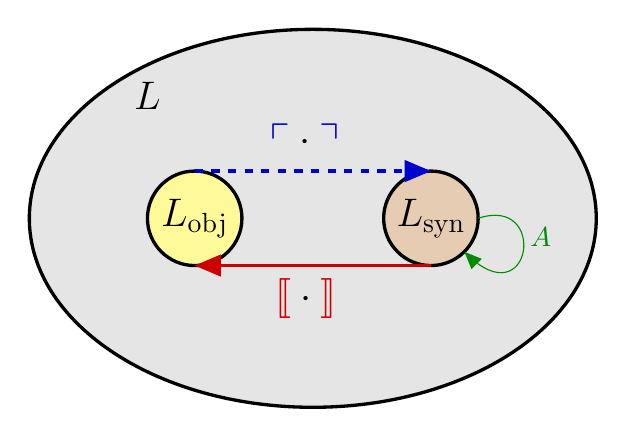
\begin{tikzpicture}[scale=.6]
  \filldraw[very thick, fill=gray!20] (3.5,0) ellipse (6 and 4);
    \draw (0,+2.6) node {\Large $L$};
  \filldraw[very thick, fill=yellow!40] (+1,0) circle (1);
    \draw (+1,0) node {\Large $L_{\rm obj}$};
  \filldraw[very thick, fill=brown!40] (+6,0) circle (1);
    \draw (+6,0) node {\Large $L_{\rm syn}$};
  \draw[-triangle 45, very thick, dashed, color=blue!80!black] (+1,+1) -- (+6,+1);
    \draw[right] (+2.4,+1.7) node {\Large $\bluesynbrack{\cdot}$};
  \draw[-triangle 45, very thick, color=red!80!black] (+6,-1) -- (+1,-1);
    \draw[right] (+2.5,-1.7) node {\Large $\redsembrack{\cdot}$};
  \draw[-triangle 45, color=green!55!black] (7,0) .. controls 
    (8.5,.5) and (8.13,-2.13) .. (6.71,-.71);
    \draw[right] (7.9,-.4) node {\bgreen{$A$}};
\end{tikzpicture}
\end{figure}
\vfill
\end{frame}

%%%%%%%%%%%%%%%%%%%%%%%%%%%%%%%%%%%%%%%%%%%%%%%%%%%%%%%%%%%%

\begin{frame}
\frametitle{{\churchqe} and {\churchuqe}}
\bi

  \item {\churchqe} is a version of Church's type theory that has a
    built-in \bblue{global reflection infrastructure}.

\ei
\end{frame}

%%%%%%%%%%%%%%%%%%%%%%%%%%%%%%%%%%%%%%%%%%%%%%%%%%%%%%%%%%%%

\begin{frame}
\frametitle{Global Reflection Infrastructure}
\vspace*{-3ex}
\vfill
\begin{figure}
\center
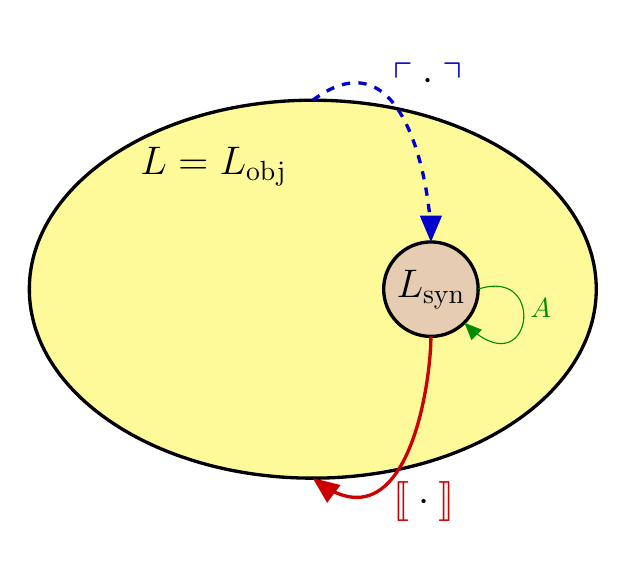
\begin{tikzpicture}[scale=.6]
  \filldraw[very thick, fill=yellow!40] (3.5,0) ellipse (6 and 4);
    \draw (+1.4,+2.6) node {\Large $L=L_{\rm obj}$};
  \filldraw[very thick, fill=brown!40] (+6,0) circle (1);
    \draw (+6,0) node {\Large $L_{\rm syn}$};
  \draw[-triangle 45, very thick, dashed, color=blue!80!black] (3.5,4) .. controls
    (5.5,5.5) and (6,2).. (6,1);
    \draw[right] (5,4.5) node {\Large $\bluesynbrack{\cdot}$};
  \draw[-triangle 45, very thick, color=red!80!black] (6,-1) .. controls
    (6,-2) and (5.5,-5.5) .. (3.5,-4);
    \draw[right] (5,-4.5) node {\Large $\redsembrack{\cdot}$};
  \draw[-triangle 45, color=green!55!black] (7,0) .. controls 
    (8.5,.5) and (8.13,-2.13) .. (6.71,-.71);
    \draw[right] (7.9,-.4) node {\bgreen{$A$}};
\end{tikzpicture}
\end{figure}
\vfill
\end{frame}

%%%%%%%%%%%%%%%%%%%%%%%%%%%%%%%%%%%%%%%%%%%%%%%%%%%%%%%%%%%%

\begin{frame}
\frametitle{{\churchqe} and {\churchuqe}}
\bi

  \item {\churchqe} is a version of Church's type theory that has a
    built-in \bblue{global reflection infrastructure}.

  \item By modifying the HOL Light proof assistant, we have produced a
    rudimentary implementation of {\churchqe} called HOL Light QE.

  \item Unlike {\churchqe}, {\churchuqe} is a variant of {\churchqe}
    that admits undefined expressions and partial functions.

  \item {\churchuqe} is well suited for specifying SBMAs that
    manipulate expressions that may be undefined such as \mname{diff}.

\ei
\end{frame}

%%%%%%%%%%%%%%%%%%%%%%%%%%%%%%%%%%%%%%%%%%%%%%%%%%%%%%%%%%%%

\begin{frame}
\frametitle{Specification of \mname{diff} in \churchuqe}
\begin{align*}
&
\ForallApp u_\epsilon \mdot\\
& \hspace*{2ex}
\If \; (\mname{DiffExpr}_{\epsilon \tarrow o} \, u_\epsilon)\\
& \hspace*{4ex}
(\mname{DiffExpr}_{\epsilon \tarrow \epsilon}(\mname{diff}_{\epsilon \tarrow \epsilon} \, u_\epsilon) \And {}\\
& \hspace*{5ex}
\bred{\ForallApp a_r \mdot}\\
& \hspace*{7ex}
\bred{{(\mname{deriv}_{(r \tarrow r) \tarrow r \tarrow r}\,(\LambdaApp x_r \mdot \sembrack{u_e}_r)\,a_r)\IsDefApp} \Implies {}}\\
& \hspace*{9ex}
\bred{\mname{deriv}_{(r \tarrow r) \tarrow r \tarrow r}\,(\LambdaApp x_r \mdot \sembrack{u_e}_r)\,a_r =
(\LambdaApp x_r \mdot \sembrack{\mname{diff}_{\epsilon \tarrow \epsilon} \, u_e}_r)\,a_r}\\
& \hspace*{4ex}
(\mname{diff}_{\epsilon \tarrow \epsilon} \, u_\epsilon)\IsUndefApp
\end{align*}
\end{frame}

%%%%%%%%%%%%%%%%%%%%%%%%%%%%%%%%%%%%%%%%%%%%%%%%%%%%%%%%%%%%

\begin{frame}
\frametitle{Future Work}
\bi

  \item Show that global reflection, as realized in {\churchqe} and
    {\churchuqe}, is a viable approach for reasoning about SBMAs.

  \item Continue the development of HOL Light QE.

  \item Define several examples of SBMAs in HOL Light QE.

  \item Prove in HOL Light QE the mathematical meanings of these SBMAs
    from their definitions.

\ei
\end{frame}

%%%%%%%%%%%%%%%%%%%%%%%%%%%%%%%%%%%%%%%%%%%%%%%%%%%%%%%%%%%%

\begin{frame}\label{lastframe}
\frametitle{Conclusion}
\bi

  \item An SBMA is an algorithm that manipulates the syntactic
    structure of expressions to achieve a mathematical task.

  \item The interplay of syntax and semantics inherent in SBMAs can
    make them tricky to implement and specify.

  \item The formal specification of SBMAs requires a reflection
    infrastructure with quotation and evaluation operators.

  \item {\churchqe} and {\churchuqe} have built-in global reflection
    infrastructures well suited for specifying, defining, and
    reasoning about SBMAs.

\ei
\end{frame}

\end{document}

\iffalse

%%%%%%%%%%%%%%%%%%%%%%%%%%%%%%%%%%%%%%%%%%%%%%%%%%%%%%%%%%%%

\begin{frame}
\frametitle{}
\bi

  \item 

\ei
\end{frame}

\fi

\end{document}
